\documentclass[12pt]{report}

\usepackage[utf8]{inputenc}
\usepackage[T1]{fontenc}
\usepackage[francais]{babel}
\usepackage{multirow}
\usepackage{array}
\usepackage{color}
\usepackage{stmaryrd}
\usepackage{fancyhdr}
\usepackage{afterpage}
\usepackage{fullpage}
\usepackage{geometry}
\usepackage{setspace}
\usepackage{enumitem}
\usepackage[hyphens]{url}
\usepackage{hyperref}
\usepackage{wrapfig}
\usepackage{float}
\usepackage{graphicx}
\usepackage{tikz}
\usepackage{varwidth}
\usepackage{listings}
\usepackage{color}
\usetikzlibrary{decorations.text}
\usepackage{enumitem}% http://ctan.org/pkg/enumitem
\definecolor{dkgreen}{rgb}{0,0.6,0}
\definecolor{gray}{rgb}{0.5,0.5,0.5}
\definecolor{mauve}{rgb}{0.58,0,0.82}
\usepackage{amsmath}
\usetikzlibrary{arrows}

\lstset{frame=tb,
  language=Java,
  aboveskip=3mm,
  belowskip=3mm,
  showstringspaces=false,
  columns=flexible,
  basicstyle={\small\ttfamily},
  numbers=none,
  numberstyle=\tiny\color{gray},
  keywordstyle=\color{blue},
  commentstyle=\color{dkgreen},
  stringstyle=\color{mauve},
  breaklines=true,
  breakatwhitespace=true,
  tabsize=3
}


% Enlève les contours des liens
\hypersetup{
    linkbordercolor={1 1 1},
    citebordercolor={1 1 1},
    urlbordercolor={1 1 1},
    colorlinks=true,
    linkcolor=black,
    urlcolor=blue
}

% Custom colors
\definecolor{green-custom}{HTML}{70ad47}
\definecolor{blue-custom}{HTML}{5b9bd5}

% Redéfinis les marges des tableaux
\let\oldtabular=\tabular
\def\tabular{\small\oldtabular}
\renewcommand{\arraystretch}{1.5}


\title{\textbf{TA72 : Simulation d'atomes}}
\author{
    Aymen DAHECH \\
        \href{mailto:dahech.aymen@utbm.fr}{aymen.dahech@utbm.fr} \and
    Anthony RUHIER \\
        \href{mailto:anthony.ruhier@utbm.fr}{anthony.ruhier@utbm.fr}
}
\date{13 janvier 2017}

\pagestyle{fancy}
\setlength{\headheight}{12pt}
\fancyhf{}
\fancyhead[L]{Aymen DAHECH, Anthony RUHIER}
\fancyhead[R]{Simulation d'atomes}
\geometry{headsep=5ex}

\graphicspath{{graphics/}}
\usetikzlibrary{arrows,positioning}

\setlength{\intextsep}{0pt}

\begin{document}

{
\newgeometry{left=1cm,right=1cm,bottom=3cm,top=1cm}
\begin{titlepage}

\vbox to 70pt{\hfill
\includegraphics[height=2cm]{logo-utbm.eps}}\
\begin{center}

\textsc{\LARGE Université de technologie Belfort-Montbéliard}\\[0.7cm]
\textsc{\LARGE Département Informatique}\\[1.0cm]
\textsc{\Large TA72 -- Projet Tutoré}\\[5cm]


% Title
{\huge \bfseries Conception d'une simulation d'atomes}\\[0.5cm]
{\huge \bfseries Rapport général}\\[3cm]

% Author and supervisor
\begin{large}
Aymen \textsc{Dahech} \\
    \href{mailto:aymen.dahech@utbm.fr}{aymen.dahech@utbm.fr}\\[1em]
Anthony \textsc{Ruhier} \\
    \href{mailto:anthony.ruhier@utbm.fr}{anthony.ruhier@utbm.fr}\\[1em]

\end{large}

\vfill

% Bottom of the page
{\large 13 janvier 2017}

\end{center}
\end{titlepage}
}

% Hack to force a new page
{\clearpage\mbox{}\thispagestyle{empty}\clearpage}
\setcounter{page}{1}

\thispagestyle{empty}
\vspace{4em}
\tableofcontents

\afterpage{\cfoot{\thepage}}
\newpage

%%%% Includes des chapitres :
%%%%%%%%%%%%%%%%%%%%%%%%%%%%%%
\setcounter{page}{1}
\chapter*{Introduction}

\addcontentsline{toc}{chapter}{Introduction}

\paragraph{}
Dans le milieu pétrochimique ou dans la chimie pédagogique, nous assistons à
une réelle demande d'outils de simulations d'éléments à vue moléculaire ou
atomique: une représentation graphique d'une réaction permet une meilleure
compréhension de celle-ci, et facilite l'apprentissage en complétant les
maquettes, souvent utilisées.

\paragraph{}
Pour répondre à ce besoin, dans le cadre de notre projet tutoré dans l'Unité de
Valeur TA72, nous avons entamé la conception d'un outil de simulations
graphique d'atomes sous la tutelle de Monsieur Fougères. Nous ne nous
démarrions pas le projet de zéro puisqu'il a également fait l'objet du projet
de fin de semestre de l'UV LP74, suite à laquelle nous nous sommes vus proposer
de le continuer.

\paragraph{}
Tel que laissé en LP74, l'outil affichait une représentation 3D d'un
environnement d'atomes, se déplaçant de manière aléatoire mais gérant les
collisions. L'utilisateur pouvait se déplacer dans l'environnement pour
visualiser les atomes. Quelques problèmes de performances étaient présents,
certains provoquant des crashs de l'application.

\chapter{Présentation du sujet}
\label{presentation_sujet}

\section{Objectifs}

\paragraph{}
Le but du projet a été de continuer le travail entrepris via la première
version de l'application afin d'obtenir trois niveaux de vues (atome, molécule
et réaction), un design en agents et des mouvements d'atomes plus réalistes qui
sont soumis à des lois d'attraction/répulsion


\section{Aperçus}

\paragraph{}
Voici différents aperçus de l'application réalisée :

\begin{figure}[H]
\centering
\centerline{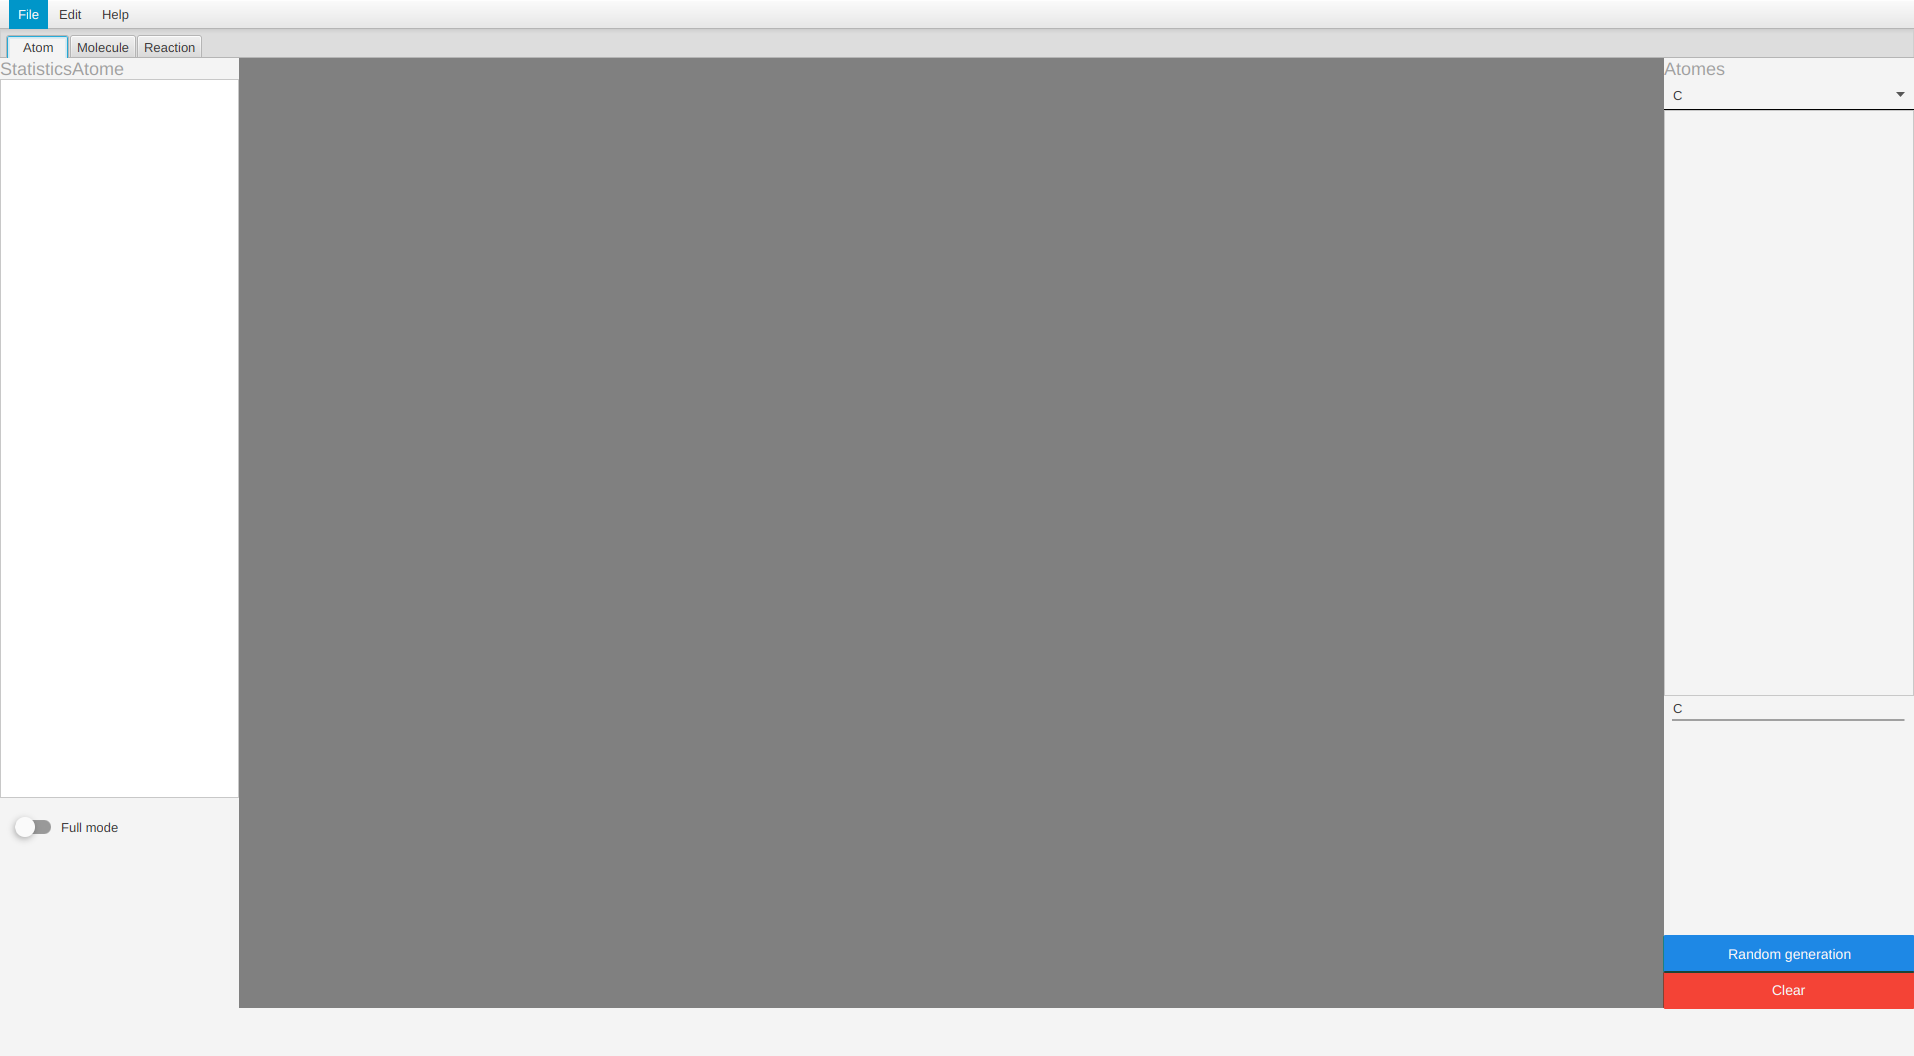
\includegraphics[width=1.2\textwidth]{screenshot_atom}}
\caption{Vue sur l'onglet Atome}
\label{screenshot_atom}
\end{figure}

\paragraph{}
La vue Atome permet normalement de générer un atome et de le visualiser.
Cependant, à la fin de cette TX, il n'est pas encore fonctionnel.

\begin{figure}[H]
\centering
\centerline{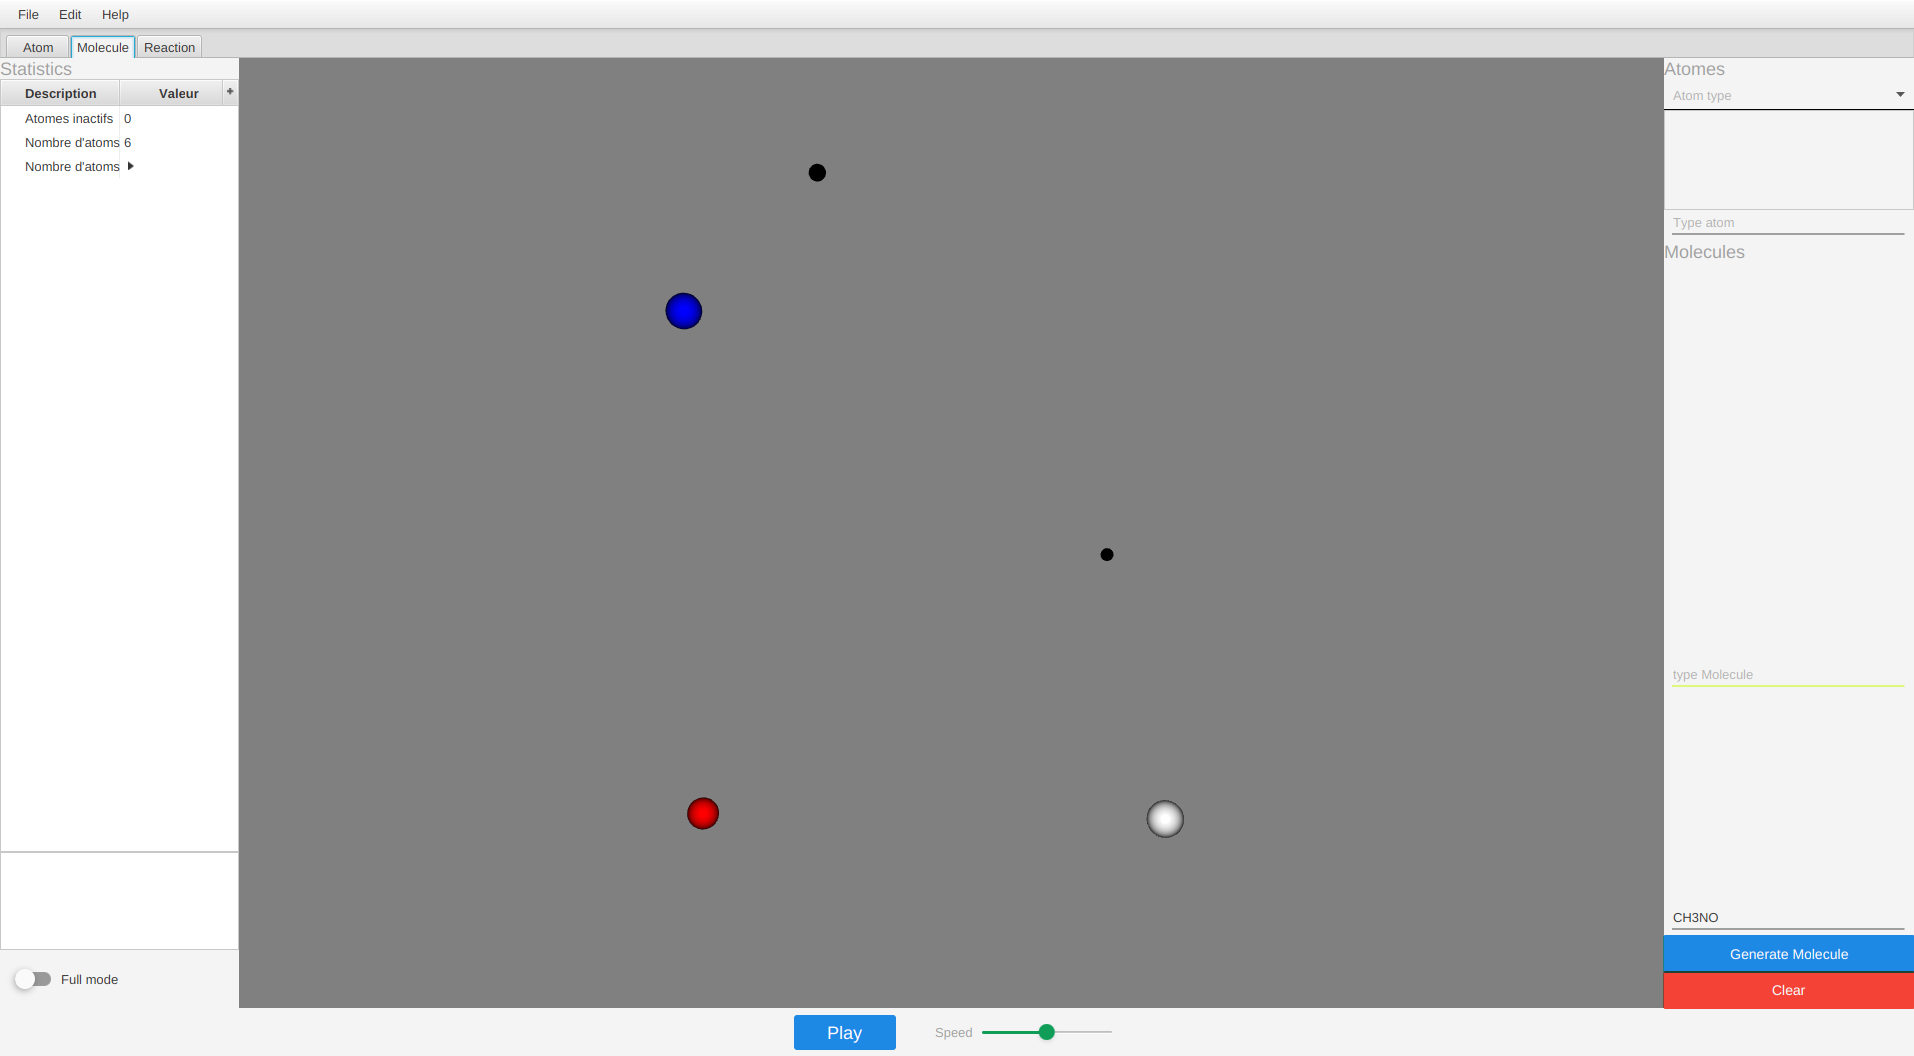
\includegraphics[width=1.2\textwidth]{screenshot_molecule}}
\caption{Vue sur l'onglet Molécule}
\label{screenshot_molecule}
\end{figure}

\paragraph{}
La vue Molécule permet de générer une molécule depuis une formule et de la
visualiser.


\begin{figure}[H]
\centering
\centerline{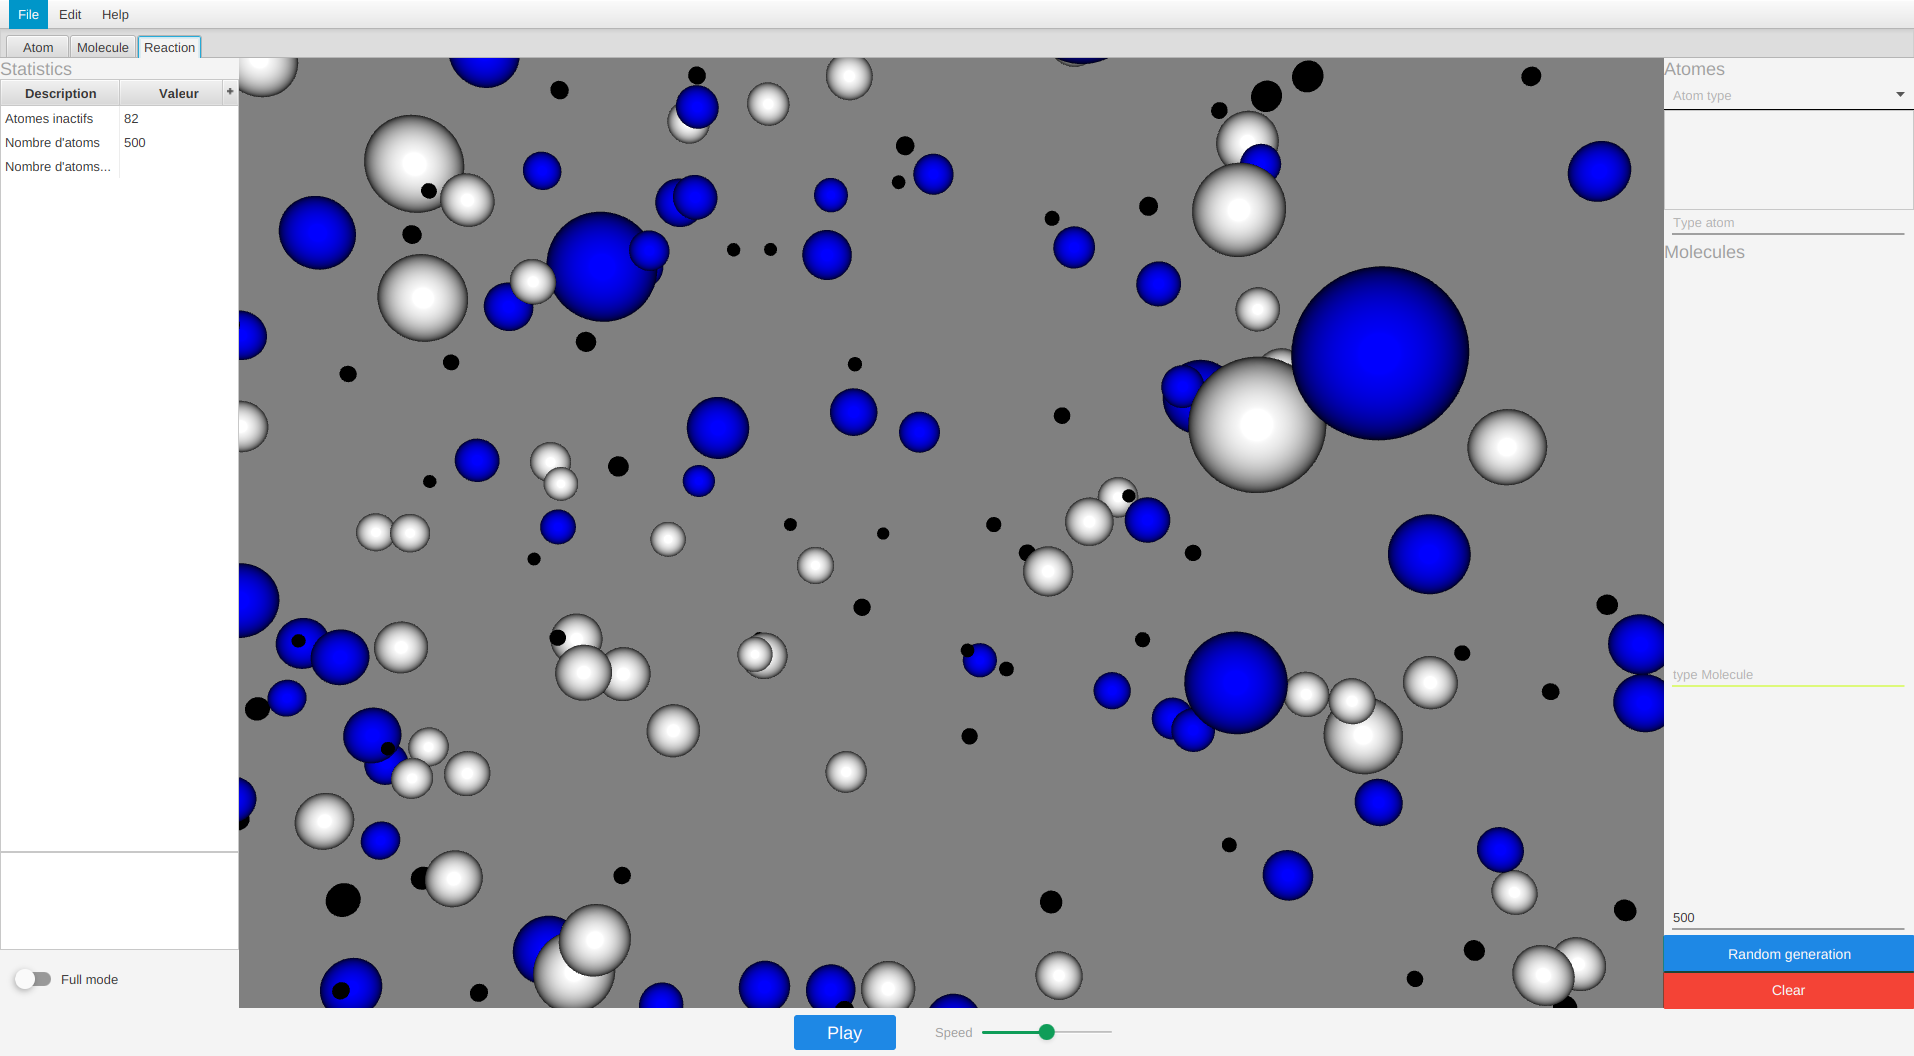
\includegraphics[width=1.2\textwidth]{screenshot_reaction}}
\caption{Vue sur l'onglet Réaction}
\label{screenshot_reaction}
\end{figure}

\paragraph{}
La vue réaction permet de générer un ensemble d'atomes, réagissant ensemble en
formant des molécules via un système d'attraction/répulsion.

\chapter{Mise en oeuvre}
\label{mise_en_oeuvre}

\section{Analyse de l'existant}

\paragraph{}
Dans une optique d'amélioration de l'existant, un bilan sur l'application telle
que rendue en LP74 a été effectué.


\subsection{Application dans un unique thread}

\paragraph{}
Le dessin des atomes, la gestion de leurs déplacements mais ainsi que toute
navigation dans l'interface sont effectués dans un unique thread.

\paragraph{}
Les atomes et molécules sont stockées dans une liste chainée, parcourue de
manière continue et séquentielle par l'application pour mettre à jour leurs
coordonnées. Il est alors nécessaire que le calcul des nouvelles coordonnées
ainsi que le dessin de chaque sphère soient simples et rapides pour rester
inférieur à la durée d'une frame, afin obtenir des mouvements fluides.

\paragraph{}
De cette manière, les atomes n'étaient pas indépendants : un objet
Environnement coordonne l'ensemble, et force de lui-même les mises à jour des
informations.  Il a également comme rôle de vérifier les collisions.


\subsection{Consommation excessive de mémoire}

\paragraph{}
L'application souffre de problèmes de consommation mémoire, avec des fuites
dues à JavaFX (le framework graphique utilisé) qui amènent des lenteurs.
L'application se fige par moments, et il arrive également qu'elle se fasse
tuer par l'OOM killer du système.


\subsection{Mouvement strictement basés sur de l'aléatoire}

\paragraph{}
Les mouvements des atomes ne sont pas basés sur des attractions ou répulsions
entre éléments. L'application impose un aspect ``brouillon'' dans les vecteurs
vitesses des éléments, de façon à donner l'impression que l'environnement n'est
pas uniforme. Tout repose sur un système aléatoire, avec gestion de collisions
et inversions de vecteurs vitesses lorsqu'un élément s'approche de trop près
des bords du bac.


\subsection{Formations de molécules}

\paragraph{}
De façon à former des molécules, et contrairement à ce qui est indiqué dans la
partie liée aux mouvements, une sorte d'attraction a été mise en place. Nous ne
considérons pas que le système en place soit suffisamment exact pour qu'il ait
une réelle influence sur les mouvements des atomes.

\paragraph{}
Néanmoins, si la vitesse d'un atome est suffisamment faible et qu'il rentre en
collision avec un autre atome, ces deux atomes vont se lier. La liaison ne
repose sur rien de scientifique, dans le sens où, par exemple, les couches de
valences ne sont pas prises en compte. Aucune vérification n'est effectuée
pour savoir si les atomes peuvent réellement se lier entre eux.

\chapter{Les modules de la simulation}
\label{les_modules_de_la_simulation}

\definecolor{mygray}{RGB}{208,208,208}
\definecolor{mymagenta}{RGB}{226,0,116}
\newcommand*{\mytextstyle}{\sffamily\Large\bfseries\color{black!85}}
\newcommand{\arcarrow}[3]{%
   % inner radius, middle radius, outer radius, start angle,
   % end angle, tip protusion angle, options, text
   \pgfmathsetmacro{\rin}{1.7}
   \pgfmathsetmacro{\rmid}{2.2}
   \pgfmathsetmacro{\rout}{2.7}
   \pgfmathsetmacro{\astart}{#1}
   \pgfmathsetmacro{\aend}{#2}
   \pgfmathsetmacro{\atip}{5}
   \fill[mygray, very thick] (\astart+\atip:\rin)
                         arc (\astart+\atip:\aend:\rin)
      -- (\aend-\atip:\rmid)
      -- (\aend:\rout)   arc (\aend:\astart+\atip:\rout)
      -- (\astart:\rmid) -- cycle;
   \path[
      decoration = {
         text along path,
         text = {|\mytextstyle|#3},
         text align = {align = center},
         raise = -1.0ex
      },
      decorate
   ](\astart+\atip:\rmid) arc (\astart+\atip:\aend+\atip:\rmid);
}
\begin{tikzpicture}
   \fill[even odd rule,mymagenta] circle (1.5);

   \node at (0,0) [
      font  = \mytextstyle,
      color = white,
      align = center
   ]{
      Atom\\
      Simulator
   };
   \arcarrow{ 85}{3}{ Atomic  }
   \arcarrow{270}{357}{ Molecular }
   \arcarrow{90}{269}{ Reaction }
\end{tikzpicture}
\section{ Module atome : présentation atomique }

\paragraph{}
Le module atome comporte la présentation atomique d'un atome selectionner. La présentation est défini dans un tableau danslequelle est indiqué le type de l'atome, son diametre, le nombre de masse (A) et le nombre atomique (Z).
la présentation d'un atome sous forme d'une sphère. Dans des prochaines amélioration, nous pouvons imaginer avoir autour de l'atome une illustration pédagogique du charge électronique.
\section{ Module molécule : formation des molécules}
\paragraph{}
Dans le module molécule, l'utilisateur peut dans un premier lieu entrer une formule chimique qui sera parser à l'aide des regex.
Une "regular expression" décrit une ou plusieurs chaînes afin de les chercher dans un corps de texte. L'expression sert de modèle pour associer un motif de caractère à la chaîne recherchée.
Une expression régulière consiste en des caractères ordinaires (par exemple, des lettres de a à z) et des caractères spéciaux, appelés métacaractères.


\begin{lstlisting}

 public ArrayList<Atom> parse(Environment environment, String formula, boolean isCHNO) {
        Pattern pattern = Pattern.compile("([A-Z][a-z]?)(\\d*)");//subdivide formula into numbers and letters such as CH2 became C, H2 or NO2Cl N,O2,Cl (the presence of a number means the end of the element)
        Matcher matcher = pattern.matcher(formula);
        ArrayList<Atom> atoms = new ArrayList<>();

        while (matcher.find()) {
            String symbole = matcher.group(2);
            Point3D a_coord;
            if (!verifyCHNO(isCHNO, matcher.group(1))) {
                continue;
}
/.../
\end{lstlisting}
\paragraph{}
Et dans une second temps, l'utilisateur peut utiliser la fonction de drag n drop afin de pouvoir constituer une molécule, les atomes vont etre placer trop proche et dans un environnment réduit, afin que la formation du molécule soit effectuer d'une maniére rapide et efficace.

\section{ Module réaction : Les interactions moléculaires}

\paragraph{}
Les interactions moléculaire sont des forces de répulsion ou d'attraction entre les molécules et les atomes non-liées. L'interaction moléculaire est trés importante dans les domaines des capteurs, conception des médicaments, nanotechnologies, etc. L'interaction moléculaire est connu aussi comme interaction non covalente ou interaction inter-moléculaire. Les interactions moléculaires ne sont pas des liaisons. Les liaisons covalantes  maintients les atomes ensembles dans les molécules . Ces liaisons se rompent et / ou se forment pendant les réactions chimiques


\subsection{Les interactions de Van der waals}
Les interactions moléculaires ont été découvertes par le scientifique néerlandais Vander Waaals. Il a remarqué que les molécules sont collantes.
L'expression «interaction de van der Waals» a signifié des forces cohésives (attraction entre les deux), des forces adhésives (attraction entre différentes) et / ou répulsives entre les molécules.

\begin{table}[h!]
\centering
 \begin{tabular}{||c | c||}
 \hline
 Atom & Van der Waals Radius \\ [0.5ex]
 \hline\hline
 H & 1.2 \\
 \hline
 C & 1.7 \\
 \hline
 N & 1.6 \\
 \hline
 O & 1.5 \\
 \hline
 \end{tabular}
\end{table}
\subsection{La formule de Lennard jones }
La formule de Lennard jones est un modèle mathématique simple qui permet de s'approcher de l'interaction entre les atomes ou des molécules neutres.
L'expression est :
 \begin{displaymath} \phi_{\rm LJ} (r) = 4\varepsilon \left[ \left(\frac{\sigma}{r}\right)^{12} - \left(\frac{\sigma}{r}\right)^{6} \right]\end{displaymath}
Oû
\begin{itemize}
    \item $\varepsilon$ est la profondeur du puit de potentiel
    \item $\sigma$ est la distance finie à laquelle le potentiel entre particule est nulle
    \item r la distance entre les partiqueme
    \item $r_m$ la distance à la quelle le potentiel atteint son minimum
\end{itemize}

A $r_m$, la fonction potentielle a la valeur de $-\varepsilon$
Le potentiel atteint son minimum autour de $r_m = 2^{\frac{1}{6}} \sigma = 1.222 \sigma$ (les distances sont liées)

Ces paramêtres peuvent etre adaptés pour reproduire  des données expérémentales ou des calculs quantique précis.
En raison de sa simplicité de calcul, le potentiel de Lennard jones est largement utilisé dans les simulations informatique meme si des potentiels plus précis existent.
L'application en mode réaction utilise cette formule dans le but de simuler le comportement inter-atomique.

Ce modèle est fortement répulsif à une ditance plus courte que le $1.222 \sigma$.
Le terme  $\sim \frac{1}{r^{12}}$, domine à courte distance, représente le modèle de répulsion entre les atoms lorsqu'ils sont trés proches. Son origine physique est liée au principe de Pauli :  quand les nuages électronique entourant les atomes commencent à ce chevaucher, l'énergie du système augmente brusquement. l'exposant 12 a été choisi exclusivement sur une base protique l'équation est facile à calculer. Sur des bases physiques, un comportement exponentiel serait plus approprié.

Le terme   $\sim \frac{1}{r^{6}}$, domine à large distance, constitue le modèle attractive. C'est le terme qui donne cohésion au système. Une attraction  $\sim \frac{1}{r^{6}}$ est produite par les forces de dispersion de van der waals. Ce sont des interactions plutôt faibles.
Les paramêtres $\sigma$ et $\varepsilon$ sont choisis pour correspondre aux propriétés physiques du matériau.

\underline{Forme simplifié de la formule :}


 \begin{displaymath}
 \phi_{\rm LJ} (r) =  \left[ \left(\frac{A}{r^{12}}\right) - \left(\frac{B}{r^{6}}\right) \right]\end{displaymath}

Oû :
\begin{itemize}
    \item $ A = 4 \varepsilon \sigma ^{12}$
    \item $ B = 4 \varepsilon \sigma ^{6}$
\end{itemize}

\subsection{L'algorithme de Verlet et les lois de Newton}

L'intégration de Verlet est une méthode numérique utilisée pour intégrer les équations de Newotn, il est fréquemment utilisé pour calculer des trajectoires de particules dans des simualtions de dynamique moléculaire et de l'infographie.
Cette intégration fournit une bonne stabilité numérique, ainsi que d'autres propriétés importantes dans les systèmes physiques telque la réversibilité temporelle sans cout de calcul supplémentaire.

\begin{displaymath} {\bf r} (t+\Delta t) = 2{\bf r} (t) - {\bf r} (t-\Delta t) + {\bf a} (t) \Delta t^2 + O(\Delta t^4) \end{displaymath}

Avec

\begin{displaymath} {\bf a} (t) = - (1/m) {\bf\nabla} V\left( {\bf r}(t) \right) \end{displaymath}

Afin de vérifier le bon déroulement de la simulation, l'application doit calculer la somme de l'énergie cinétique K et  V qui doit égale à E  ($ E = K + V $)
\subsection{Le module physique dans l'application}
Chaque atome dans la simulation se déplace simplement en réponse aux forces exercées par les atomes proches et les murs de l'environnement, conformément aux lois du mouvement de Newton. L'algorithme ne connait ni les transformations de phase, ni l'irréversibilité mais ces phénomènes de haut niveau et d'autre émergent de la physique microscopique.

La force entre les atomes est calculée à partir de la formule de Lennard jones.La simulation se rapproche des lois de newton en utilisant l'algorithme de Verlet avec l'étape de temps. L'utilisation d'un pas de temps trop important peut rendre la simulation inexacte et parfois meme instable.
L'application utilise un system naturel d'unité, avec le diamètre atomique, la masse atomique, le profondeur de potentiel de Lennard Jones et la constante de Boltzmann.

\chapter{ Implémentation d'agent }
\label{Implementation_d_agent}
\paragraph{}
Les agents sont considérés comme l'un des paradigmes les plus importants qui peuvent améliorer les méthodes actuelles de conceptions. Le terme "Agent" a trouvé son chemin dans un certain nombre de technologie et a été largement utilisé, par exemple, dans l'intelligence artificielle, les bases de données, les systèmes d'explorations, etc. Un agent est essentiellement un composant logiciel spécial qui possède une autonomie. Un agent est un systèm solidaire qui travail dans un environnement. Les systèmes multi-agents peuvent modéliser des systèmes complexes. les agents dans ce système agisse les un sur les autres. Un agent est autonome et proactif qu'il n'agit pas simplement en réponse à son environnement mais est capable d'afficher un comportement orienté vers l'objectif en prenant l'initiative (autonomous behavior).

\section{ Jade }
\subsection{Jade architecture}
\paragraph{}
Jade est composée de conteneurs d'agents qui peuvent être distribués sur le réseau. Les agents vivent dans des conteneurs qui sont le processus java qui fournit le temps d'exécution de JADE et tous les services nécessaires pour héberger et exécuter des agents. Il y a un conteneur spécial, appelé conteneur principal, qui représente le point d'amorçage d'une plate-forme: c'est le premier conteneur à lancer et tous les autres conteneurs doit se joindre à un conteneur principal (main container) en s'inscrivant avec lui.
\paragraph{}
JADE est un middleware qui facilite le développement de systèmes multi-agents en vertu de la norme FIPA pour laquelle il crée de multiples conteneurs pour les agents, chacun d'eux peut fonctionner sur un ou plusieurs systèmes. Il est entendu qu'un ensemble de conteneurs constitue une plate-forme.

JADE propose:
\begin{itemize}
    \item Un environnement où les agents JADE sont exécutés.
    \item Bibliothèques pour créer des agents utilisant l'héritage et la redéfinition des comportements.
    \item Une boîte à outils graphique pour le suivi et la gestion de la plate-forme d'agents intelligents.

\end{itemize}


\subsection{Le cycle de vie d'agent JADE}
\paragraph{}
Le cycle de vie d'un agent JADE suit le cycle proposé par FIPA. Ces agents passent par différents états définis comme:
\begin{itemize}

    \item Initié: l'agent a été créé.
    \item Active: L'agent a été enregistré et a un nom. Dans cet état, il peut communiquer avec d'autres agents.
    \item Suspendu: l'agent est arrêté parce que son thread est suspendu.
    \item Attente: l'agent est bloqué en attente d'un événement.
    \item Supprimé: L'agent a terminé et son thread a terminé son exécution.
    \item Transit: l'agent se déplace vers un nouvel emplacement.
\end{itemize}

\paragraph{}
\section{Gui Agent}
Dans notre application, l'interface graphique est un agent. Cet agent au moment d'initialisation il crée un conteneur d'agent "sink-container". Ce contenair servira comme bassin pour les controlleurs ( chaque module; atome, molécule et réaction; est un agent sont missions principales est d'assurer le bon déroulement de la simulation.


\usetikzlibrary{arrows.meta}
\tikzset{%
  >={Latex[width=2mm,length=2mm]},
  % Specifications for style of nodes:
            base/.style = {rectangle, rounded corners, draw=black,
                           minimum width=4cm, minimum height=1cm,
                           text centered, font=\sffamily},
  activityStarts/.style = {base, fill=blue!30},
       startstop/.style = {base, fill=red!30},
    activityRuns/.style = {base, fill=green!30},
         process/.style = {base, minimum width=2.5cm, fill=orange!15,
                           font=\ttfamily},
}


\begin{lstlisting}

//ApplicationAgent.java
public class ApplicationAgent extends Agent {
    /** setting up agent **/
    @Override
    public void setup() {
        System.setProperty("prism.dirtyopts", "false");
        Application.launch(FactoryGui.class);
    }
}
//FactoryGui.java
public class FactoryGui extends Application {
    /** Gui Agent start : define agent profile, create container for the controllers agents */
    @Override
    public void start(Stage stage) throws Exception {
        Runtime rt = Runtime.instance();
        /.../
        pc.setParameter(Profile.LOCAL_HOST, "127.0.0.1");
        pc.setParameter(Profile.CONTAINER_NAME, "sink-container");
        pc.setParameter(Profile.NO_MTP, "true");
        AgentContainer container = rt.createAgentContainer(pc);
        /.../
            FXMLLoader f = new // setting up the Gui FXMLLoader(ApplicationAgent.class.getClassLoader().getResource(("uiAtoms.fxml")));
            Parent parent = f.load();
            c = f.getController();
            c.setParent(parent);
            c.setContainer(container);//creating controllers container
            container.acceptNewAgent("controller", c);//adding main controller in the container
            c.AStart(stage, true);
            /.../

    }
}
\end{lstlisting}

\section{Controller agent}
\paragraph{}
Le main controlleur a pour mission le bon fonctionnement de GUI, il initialise les autres controlleurs (chaque tab a son propre controlleur qui assure le fonctionnement de ce tab). Ces controlleurs créer les environnements ou se déroulera la réaction. Chaque environnement est un container qui recevra les différents atomes sous forme d'agent.



\begin{tikzpicture}[node distance=1.5cm,%
    every node/.style={fill=white, font=\sffamily}, align=center]

  \node (start)             {Application agent starts};
  \node (masterController)     [process, below of=start]          {Controller (MASTER)};
  \node (AtomController)      [process,left of=masterController, xshift=-4cm]   {Atom Controller};
  \node (MolecularController)      [process,right of=masterController, xshift=4cm]   {Molecule Controller};
  \node (ReactionController)      [process, below of=masterController]   {Reaction Controller};

  \node (atom1)     [process, below of=AtomController]   {Atom ex: H};
  \node (Environment)      [activityRuns, below of=ReactionController]
                                                      {Create Environment};

  \node (atoms)     [activityRuns, yshift=-2cm, below of=Environment]   {Atoms as agents};


  \draw[->]     (start) -- (masterController);
  \draw[->]     (masterController) -- (AtomController);
  \draw[->]     (masterController) --(MolecularController);
  \draw[->]     (masterController) --  (ReactionController);
  \draw[->]     (ReactionController) --  (Environment);
  \draw[->]     (MolecularController) |-  (Environment);
  \draw[->]     (AtomController) --  (atom1);
  \draw[->]     (atom1) |- node[text width=3cm]
                                   {Add atom to environment}  (Environment);
  \draw[->]     (Environment) -- node[text width=3cm]
                                   {contain agents}(atoms);
\end{tikzpicture}

\section{Atom agent}
\paragraph{}
Chaque atome dans notre application est considéré comme un agent. Il a un cycle de vie composé de quatres phase:
\begin{itemize}
\item Phase d'initialisation (setup) : dans laquelle, l'atome initialise ces propriétés (vitesse, symbole, rayon de van der waals ...)
\item Phase de démarrage : dans la quelle il va rejoindre le conteneur d'agent est déclenché son comportement.
\item Phase de vitalité : dans la quelle l'atome a son propre comportement selon un modèle chimico-physique à l'aide des différent algorithme a bordé dans la section simulation moléculaire.
\item Phase de destruction : l'agent sera retiré du conteneur d'agent et détruit de la simulation.
\end{itemize}


\begin{figure}[H]
\centering
\centerline{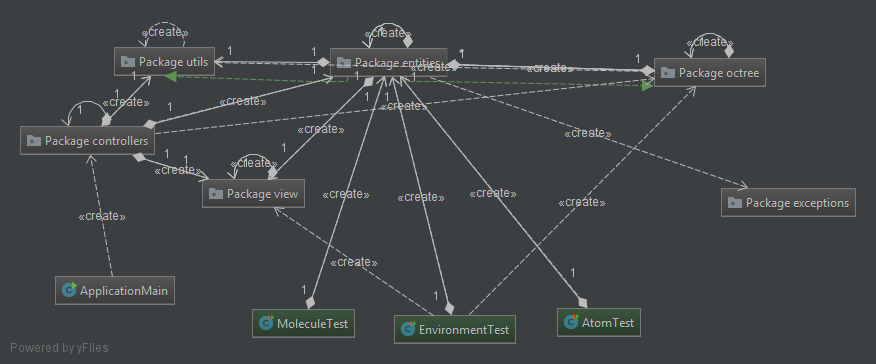
\includegraphics[width=1\textwidth]{diagram.png}}
\caption{Diagrame de dépendenc }
\label{diagram_im}
\end{figure}

\chapter{Datastructure Octree}
\label{mise_en_oeuvre}

\paragraph{}
Pour la gestion des collisions et l'attraction/répulsion, la recherche du plus
proche voisin est utilisée pour chaque atome et pour chaque frame. Avec la
datastructure utilisée pour stocker les atomes (une ArrayList), pour chaque
atome on a alors une complexité en pire scénario de $O(N)$. Au total, pour tous
les atomes, on a alors une complexité en $O(N^2)$ pour chaque frame.

\paragraph{}
Dans l'ancienne implémentation séquentielle, la liste des atomes était
parcourue pour chaque frame de façon à mettre à jour les positions des atomes.
Utiliser une datastructure pour optimiser la recherche de voisins augmenterait
dans tous les cas la complexité du parcours des atomes. Le passage sur des
atomes Agents a changé la donne, puisqu'ils se mettent à jour eux même et
évitent le parcours de liste. Il y a alors tout intérêt à opter pour une
datastructure plus optimisée pour la recherche que pour le parcours.


\section{Choix de datastructure}

\paragraph{}
La nouvelle datastructure pour stocker les atomes se doit d'être optimisée pour
la recherche de voisins dans un environnement 3D. Les deux datastructures qui
ressortent sont l'Octree et le K-D Tree.

\subsection{Octree}

\paragraph{}
Un Octree est la version tridimensionnelle du Quadtree, reposant sur la
sous-division de cubes en 8 cubes enfants. Un cube contient un nombre
d'éléments maximum M. Dès que ce nombre est dépassé, le cube se subdivise en 8
cubes.

\begin{figure}[H]
\centering
\centerline{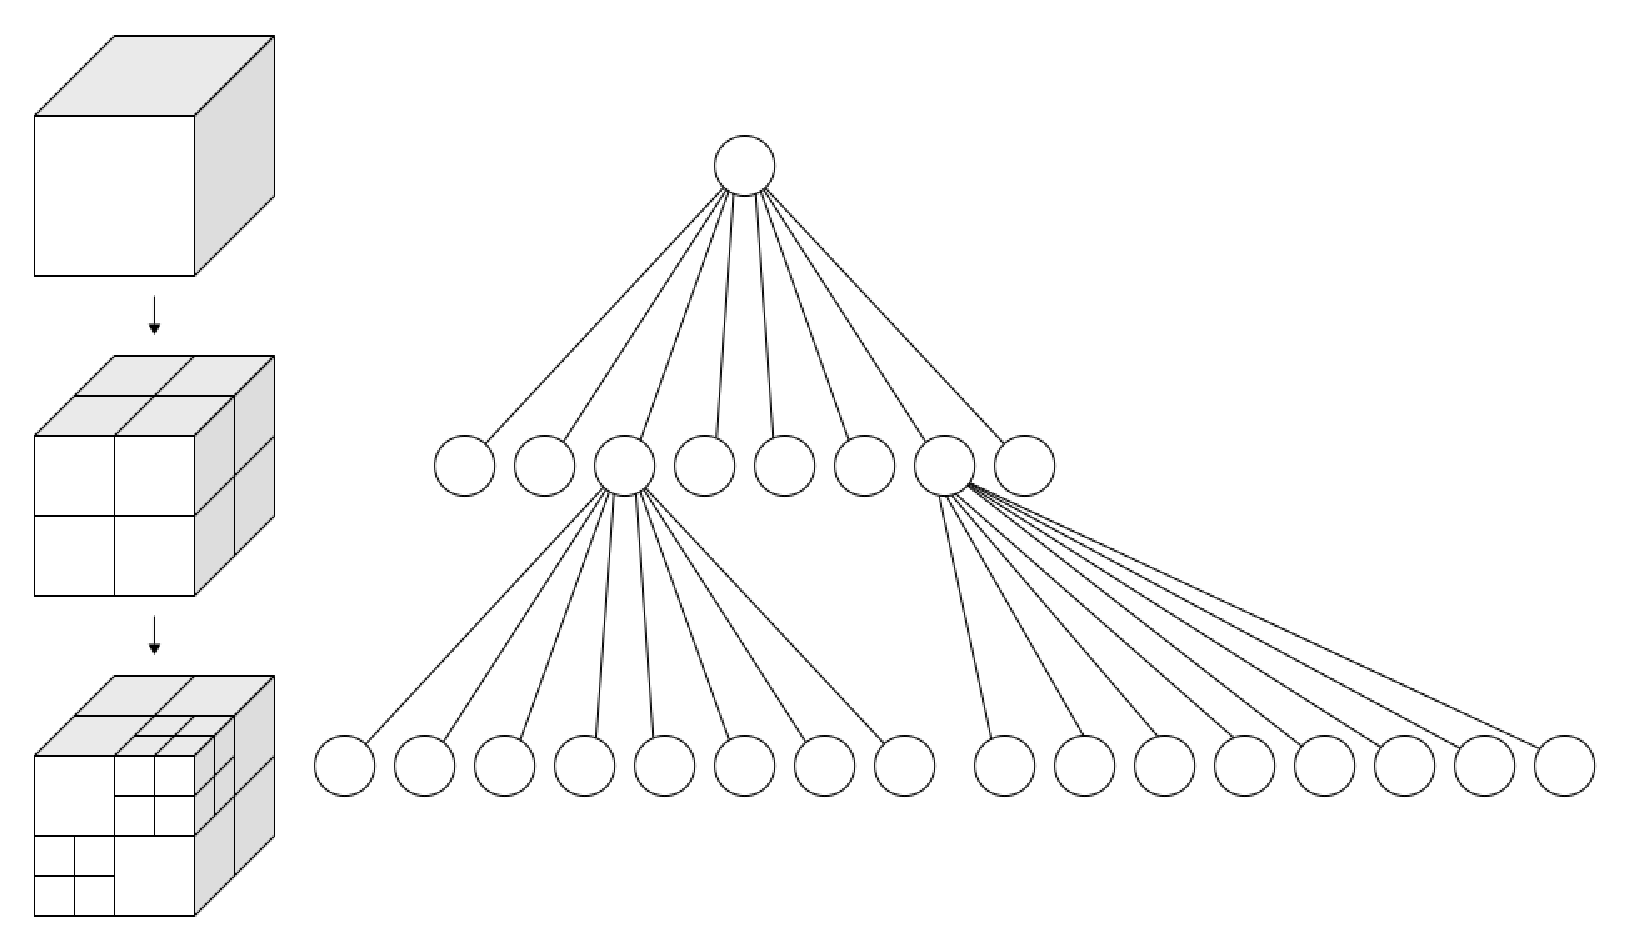
\includegraphics[width=0.8\textwidth]{octree.eps}}
\caption{Schéma de décomposition d'un octree}
\label{octree_img}
\end{figure}

\paragraph{}
Après sous-division, les objets sont éparpillés dans les cubes enfants en
fonction de leur position dans l'espace. Il s'agit, pour simplifier, de classer
les objets via une sorte de dichotomie pour chaque dimension, d'où les 8 cubes.
La recherche d'un élément via ses coordonnées est alors très rapide, puisque
les éléments sont disposés dans chaque cube en fonction de cette variable.


\subsubsection{Recherche de voisins}
\paragraph{}
Dans chaque cube, les éléments sont stockés dans une ArrayList de taille
maximum $M$, fixée et comprise entre 1 et $N$ ($N$ le nombre total d'éléments
stockés dans l'ensemble de l'octree). La recherche de voisins s'effectue en
cherchant les cubes entourant un objet. La recherche du plus proche voisin a
alors comme complexité dans le pire cas $O(27(M + N))$, soit environ $O(M+N)$.
$O(M)$ est ici la complexité à parcourir tous les éléments de chaque cube
(puisque cela revient à parcourir une ArrayList de taille $M$). $O(N)$
correspond à la complexité à atteindre un cube donné dans l'octree dans le pire
des cas. Ces deux complexités sont à multiplier par 27, qui correspond au
nombre maximum de cubes pouvant entourer un objet. Dans le cas où $M$ est fixée
à la même valeur que $N$, la complexité est de $O(2N)$ par atome, soit $O(N^2)$
pour avoir le plus proche voisin pour l'ensemble des $N$ atomes.

\paragraph{}
Le cas moyen est intéressant à étudier car montre le rôle que joue M dans
l'efficacité de l'algorithme. La complexité est de $O(M +
\frac{\log(N)}{3\log(M)\times{}\log(2)})$, soit environ $O(M +
\frac{\log(N)}{\log(M)})$. On négligera le nombre de cubes entourant l'élément
puisqu'il n'impacte que peu la complexité finale. $O(M)$ est ici encore la
complexité à parcourir tous les éléments d'un cube (ArrayList de taille $M$).
$O(\frac{\log(N)}{\log(M)})$ correspond ici à la complexité d'accéder à un cube
donné. Le nombre de cubes moyen entourant un objet est ici négligé. Si $M$ se
rapproche de 1, la complexité est environ de $O(N)$ par atome, soit $O(N^2)$
pour l'ensemble des atomes. La complexité est environ la même si $M = N$.
Néanmoins, il est plus avantageux que $M$ soit égal à $N$ plutôt qu'à 1, à
cause du nombre de cubes entourant l'objet pas mis en évidence ici car non pris
en compte dans les calculs.

\paragraph{}
On s'aperçoit alors que l'Octree est avantageux pour la recherche de voisins,
mais il est important de fixer une valeur appropriée pour le nombre maximum
d'éléments par cube, auquel cas la complexité sera plus mauvaise que celle
d'une ArrayList. Fixer un $M$ trop faible reviendra à obtenir énormément de
cubes, puisqu'un cube ne pourra contenir que peu d'éléments, ce qui rendra lent
l'accès à un cube donné. Fixer un $M$ trop proche de $N$ rendra l'octree
inefficace, car sera composé de très peu de cubes contenant un grand nombre
d'éléments.


\subsubsection{Déplacement d'éléments}
\paragraph{}
Les nœuds de l'arbre dépendent des coordonnées des points, donc déplacer un
point peut amener à déplacer un nœud. Contrairement à l'arbre k-d, cette étape
n'est pas forcément nécessaire, et le déplacement léger d'un atome ne
requièrera pas, dans la plupart des cas, d'être déplacé dans un autre cube.  On
aura alors dans la plupart des cas une complexité de $O(1)$ pour le déplacement
d'un atome, et au pire $O(N)$ ($O(2N)$ pour accéder au cube de l'élément à
déplacer puis le supprimer de l'ArrayList, $O(2N)$ pour l'insérer dans le cube
approprié à ses nouvelles coordonnées). Également, un octree n'a pas besoin
d'être équilibré. Ces deux points en font un arbre intéressant pour le cas de
la simulation d'atomes, où les éléments sont sans cesse en mouvement.


\subsubsection{Choisi comme datastructure principale}
\paragraph{}
L'octree a été choisi comme datastructure servant à stocker ses atomes pour sa
facilité d'implémentation comparé à un arbre k-d, la rapidité en moyenne à
déplacer un élément et la complexité de la recherche de voisin le plus proche,
qui permet d'être au pire quasiment aussi efficace qu'une ArrayList, et dans le
meilleur des cas permet de se rapproche d'une complexité en $O(\log(N))$ par
élément, soit $O(N\log(N))$ pour l'ensemble des atomes, lorsque la variable $M$
est correctement fixée et $N$ assez grand.

\subsection{K-D Tree}

\paragraph{}
Un K-D tree est un arbre binaire, équilibré. La complexité en cas moyen pour de
la recherche de voisins est de $O(log(N))$, pire cas $O(N)$. Comme pour
l'octree, les nœuds de l'arbre dépendent des coordonnées des points, donc ici
déplacer un point revient à déplacer un nœud et à re-balancer l'arbre. Ce point
est important car nous sommes ici dans un environnement où les atomes sont
constamment en mouvement.  La complexité d'insertion d'élément est en moyenne
de $O(log(N))$, ce qui est également le cas pour la suppression. Bouger un
élément dans l'arbre a alors une complexité de $O(2log(N))$.

\paragraph{}
Pour chaque frame, en cas moyen, la méthode de recherche de voisin ainsi que le
déplacement d'atome aurait une complexité de $O(3log(N))$, et comme pire cas
$O(3N)$. Au total, pour tous les atomes, la complexité totale serait alors de
$O(Nlog(N))$ en cas moyen et $O(N^2)$ en pire cas. Cela reste inférieur à la
complexité de l'ArrayList en cas moyen, mais il faut atteindre un grand nombre
d'atomes pour que la différence soit intéressante, c'est pourquoi la solution
n'a pas été retenue.

\chapter*{Conclusion}

\addcontentsline{toc}{chapter}{Conclusion}

\paragraph{}


\end{document}
